%Custom Functions
\newcommand{\CompanyName}{TT} % update later

\documentclass[conference]{IEEEtran}
\IEEEoverridecommandlockouts
% The preceding line is only needed to identify funding in the first footnote. If that is unneeded, please comment it out.
%\usepackage{cite}
\usepackage{amsmath,amssymb,amsfonts}
\usepackage{algorithmic}
\usepackage{graphicx}
\usepackage{textcomp}
\usepackage{xcolor}

\usepackage{pdflscape}

\usepackage[utf8]{inputenc}
\usepackage{fancyhdr}
\usepackage{lastpage}

% Please add the following required packages to your document preamble:
\usepackage{multirow, makecell, rotating}
\usepackage[numbers]{natbib}

\usepackage{listings}
\usepackage{hyperref}
\usepackage{amsmath}


\hypersetup{
    citecolor=black,
    colorlinks=true,
    linkcolor=black,
    filecolor=magenta,      
	urlcolor=cyan
}

\usepackage{listings}
\usepackage{color}

\definecolor{dkgreen}{rgb}{0,0.6,0}
\definecolor{gray}{rgb}{0.5,0.5,0.5}
\definecolor{mauve}{rgb}{0.58,0,0.82}

\lstset{frame=single,
  language=C++,
  showstringspaces=false,
  columns=flexible,
  basicstyle={\small\ttfamily},
  numbers = none,
  numberstyle=\tiny\color{gray},
  keywordstyle=\color{blue},
  commentstyle=\color{dkgreen},
  stringstyle=\color{mauve},
  breaklines=true,
  breakatwhitespace=true,
  tabsize=2
}

\def\BibTeX{{\rm B\kern-.05em{\sc i\kern-.025em b}\kern-.08em
T\kern-.1667em\lower.7ex\hbox{E}\kern-.125emX}}

\fancypagestyle{fancylandscape}{
\fancyhf{} %Clears the header/footer
\fancyfoot{% Footer
\makebox[\textwidth][r]{% Right
  \rlap{\hspace{.75cm}% Push out of margin by \footskip
    \smash{% Remove vertical height
      \raisebox{4.87in}{% Raise vertically
        \rotatebox{90}{Page \thepage\ of \pageref{LastPage}}}}}}}% Rotate counter-clockwise
\renewcommand{\headrulewidth}{0pt}% No header rule
\renewcommand{\footrulewidth}{0pt}% No footer rule
}

\pagestyle{fancyplain}
\fancyhf{}
\fancyfoot[c]{Page \thepage\ of \pageref{LastPage}}
\renewcommand{\headrulewidth}{0pt}

\begin{document}

\title{A Risky Coexistence: Examining the Challenges Faced by Autonomous Vehicles and Motorcycles}

\author{\IEEEauthorblockN{1\textsuperscript{st} Given Edward Patch}
	\IEEEauthorblockA{\textit{Software Engineering and Artificial Intelligence (of MSc Year 4)} \\
		\textit{Autonomous Vehicle Research}\\
		\textit{University of Wales Trinity St. Davids (of Dr. Tim Bashford)}\\
		Swansea, Wales \\
		Student ID: 1801492}}

\maketitle
\thispagestyle{plain}
\pagestyle{plain}

\begin{abstract}

\end{abstract}

\begin{IEEEkeywords}
	
\end{IEEEkeywords}

\section{Introduction}
	 Autonomous Vehicles (AVs) are scheduled to roll out to the United Kingdom roads by 2025.~\cite{govuk_self-driving_2022} With the rise of automated vehicles, a safety concern arises, which affects the development of AVs, including government bodies and manufacturers, public safety and the National Health Service (NHS), when it comes to motorcycles and AVs. The research focuses on issues that may have been overlooked already with motorcycles, with new scenarios introduced in many US states, like road widths, filtering and poor weather conditions with British vehicles. 

	Addressing these issues could be problematic; however, with Object Classification, which is not entirely accurate compared to AV standard, the research could push more extensive research in this area. The study's objectives are to understand the existing dangers with AVs and motorcycles, establish appropriate datasets to train and test the selected models, remove any vehicles that are not necessary for the study, and evaluate the test results of the study.
	
	A few study results are showcased to illustrate the current issues that may arise, describing the reasoning the model may have not detected. These results will be cross-referenced to research that did similar tests to support the argument to drive the safety issues that may still exist with AV manufacturers or newly established UK AV manufacturers.

\section{Literature Review}

\section{Methodology}
	\subsection{Objectives}
	The main objectives of this project are to develop an accurate FER model using CNNs and to improve the model's performance on specific tasks. The following steps be undertaken to achieve these objectives:-

	\begin{enumerate}
		\item Dataset Preparation: Object Classification requires a set of labels to correspond to an image, mapping different classified objects wihin the image. Preparation of the data requires being able to select validated data for training and testing purposes.
		\item Pre-processing: Read in the mapping datasets and extract the sorted datasets to the designated file paths. 
		\item Architecture Selection and Optimisation: Investigate different object classification architectures, and select a model that could cloisely demonstrate an idea of how Autonomous Vehicles currently initialise object classification.
		\item Evaluation Techniques: A few methods to analyse and evaluate the model's performance and accuracy regarding the learning and predictive classifications. Classification Reports and Confusion Matrices to identify optimisation issues to improve accuracy results. Training and validation evaluation methods are required to determine the model's learning quality. The Python libraries involved includes history when a model is fitted, which includes `loss' and `val\_loss' to determine the optimisation of the learning state of the model. An evaluation of validation data is essential to highlight any errors within the preparation phase.
	\end{enumerate}

	\subsection{Pre-Processing}
	\label{subsec:preprocessing}
		Using Python scripts, the selected training material is taken and processed together, allowing the model to see different motorcycles in different scenarios. A US and Indian dataset was used to get different road conditions and different types of motorcycles. Using the two datasets helped increase the accuracy during the validation process.

		Training of two datasets, dataset A with the filter of `bus', `car', `minivan', `motorcycle', `pickup', `scooter', `trike', `truck', `van', `person', whereas dataset B involves; `motorcycle', `tricycle' and `person' filters. The `yolov5s.pts' and `yolov5l.pts' were used during testing, with better results on the `yolov5l.pts' by 25\% when identifying motorcycles. Both weights used a batch of thirty-two and ten epochs.

		Testing materials must include video content, split into multiple frames To test the trained YOLO model, with enough images to create a strong argument. Joining a motorcycle group and exploring various routes across the United Kingdom, including motorways, dual carriageways, A-roads, and backroads, with motorcycles overtaking, filtering, and navigating blindspots, can lead to unexplored scenarios and questions that may have been previously overlooked.
					
		A decided factor is to use a Drift Innovation Ghost XL motorcycle camera attached to a motorcycle that rides within the group, then swap the camera with another rider after some time. This way, combining the content helps identify how Object Classification copes with numerous blindspots and draws some questions to further the research concerning the current safety of AV vehicles. 
		
		One sports bike and two cruisers are selected for material to test how Object Classification models handle different motorcycle styles. Ideal footage would include Scramblers, Trikes and other similar vehicles to establish how Object Classification models work in an estimated manner. A perfect material would be that during the ride out, conducted on 18$^\text{th}$ July 2023, Tuesday, would capture these vehicles, which either pass by or join us in sections of the rides. The group is instructed to overtake and be undertaken by the camera vehicle to create plenty of footage to put the YOLO model to the test. However, it is worth noting that no rider is pressured into doing anything illegal or unsafe.

	\subsection{Model Architecture}
		With the challenge of setting up a high-end model equivalent to a leading AV manufacturer like Tesla, it is essential to use detailed Object Classification training material. Using the Qualitative Research method with video frames and labels to classify the different objects in the video is required. Roboflow and other materials are outsourced and looked into using different sources found in various research journals.

\section{Results}
	\subsection{YOLOv5 Architecture | YOLOv5 Large Weight | Dataset A}
		\begin{figure}[h]
			\centering
			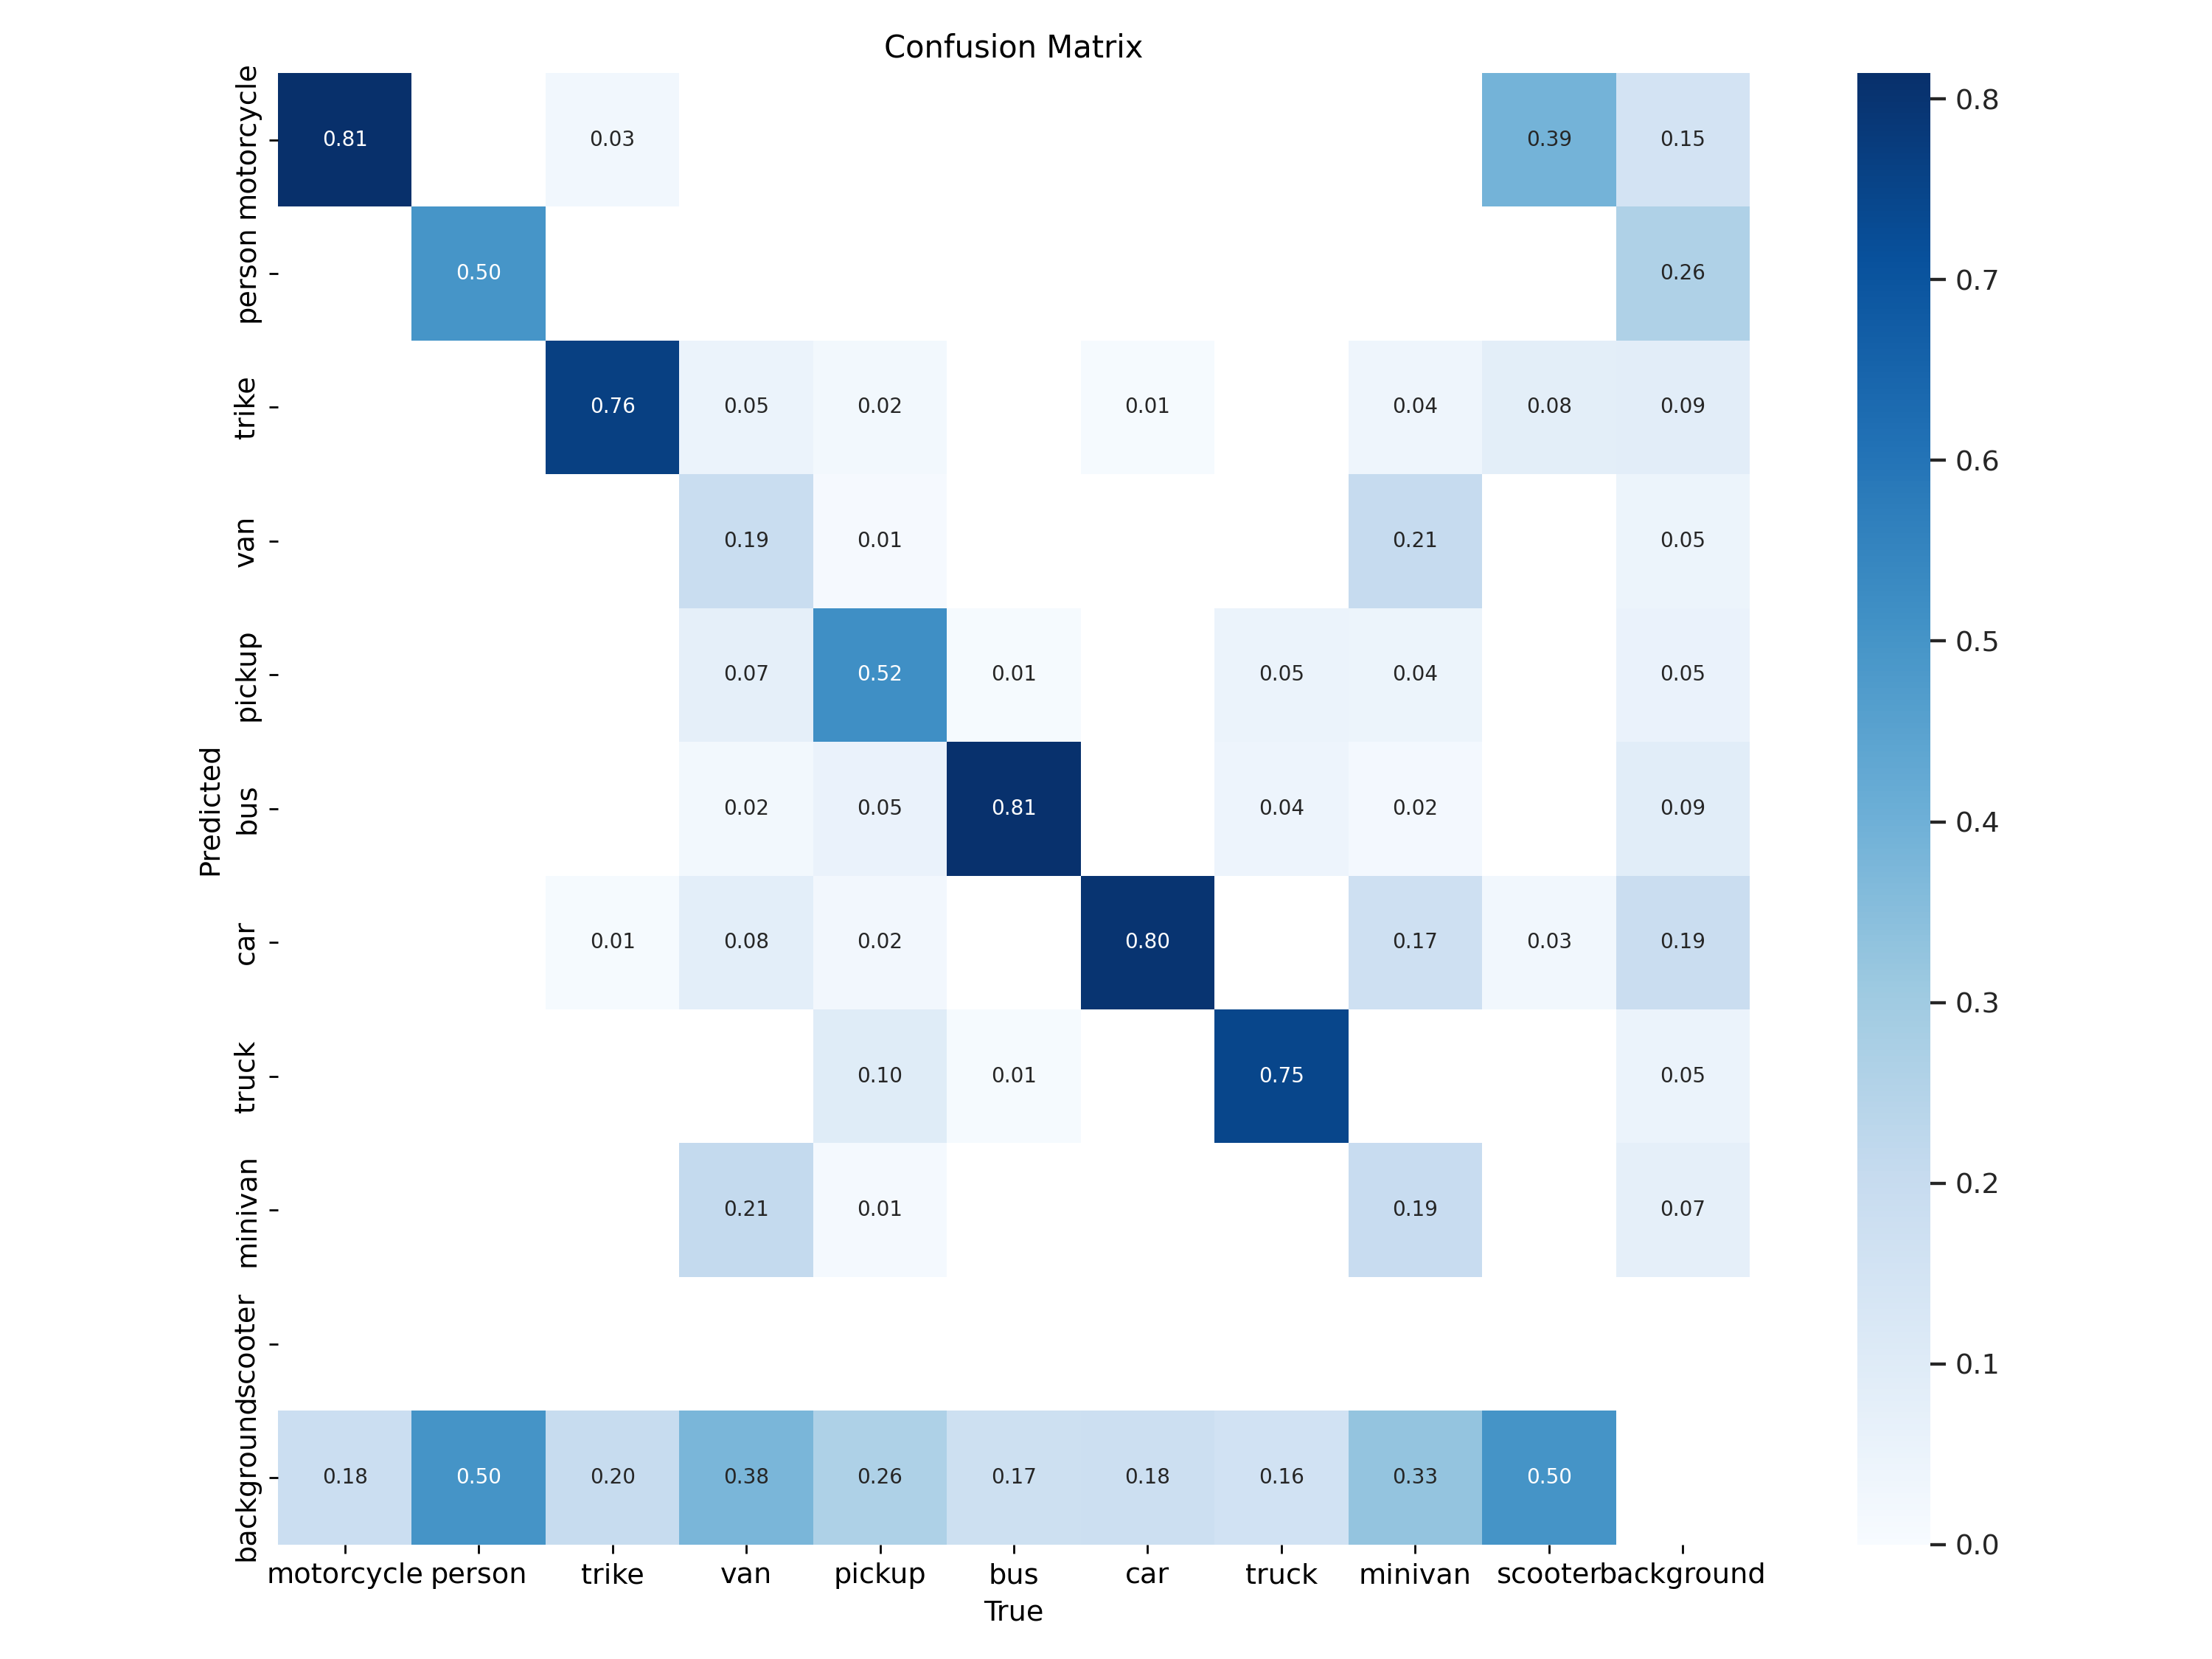
\includegraphics[width=\columnwidth]{Figures/a_confusion_matrix.png}
			\caption{Dataset A: Confusion Matrix of YOLOv5 model}
			\label{fig:ukDatasetYolov5LargeWeight}
		\end{figure}

	\subsection{YOLOv5 Architecture | YOLOv5 Large Weight | Dataset B}
		\begin{figure}[h]
			\centering
			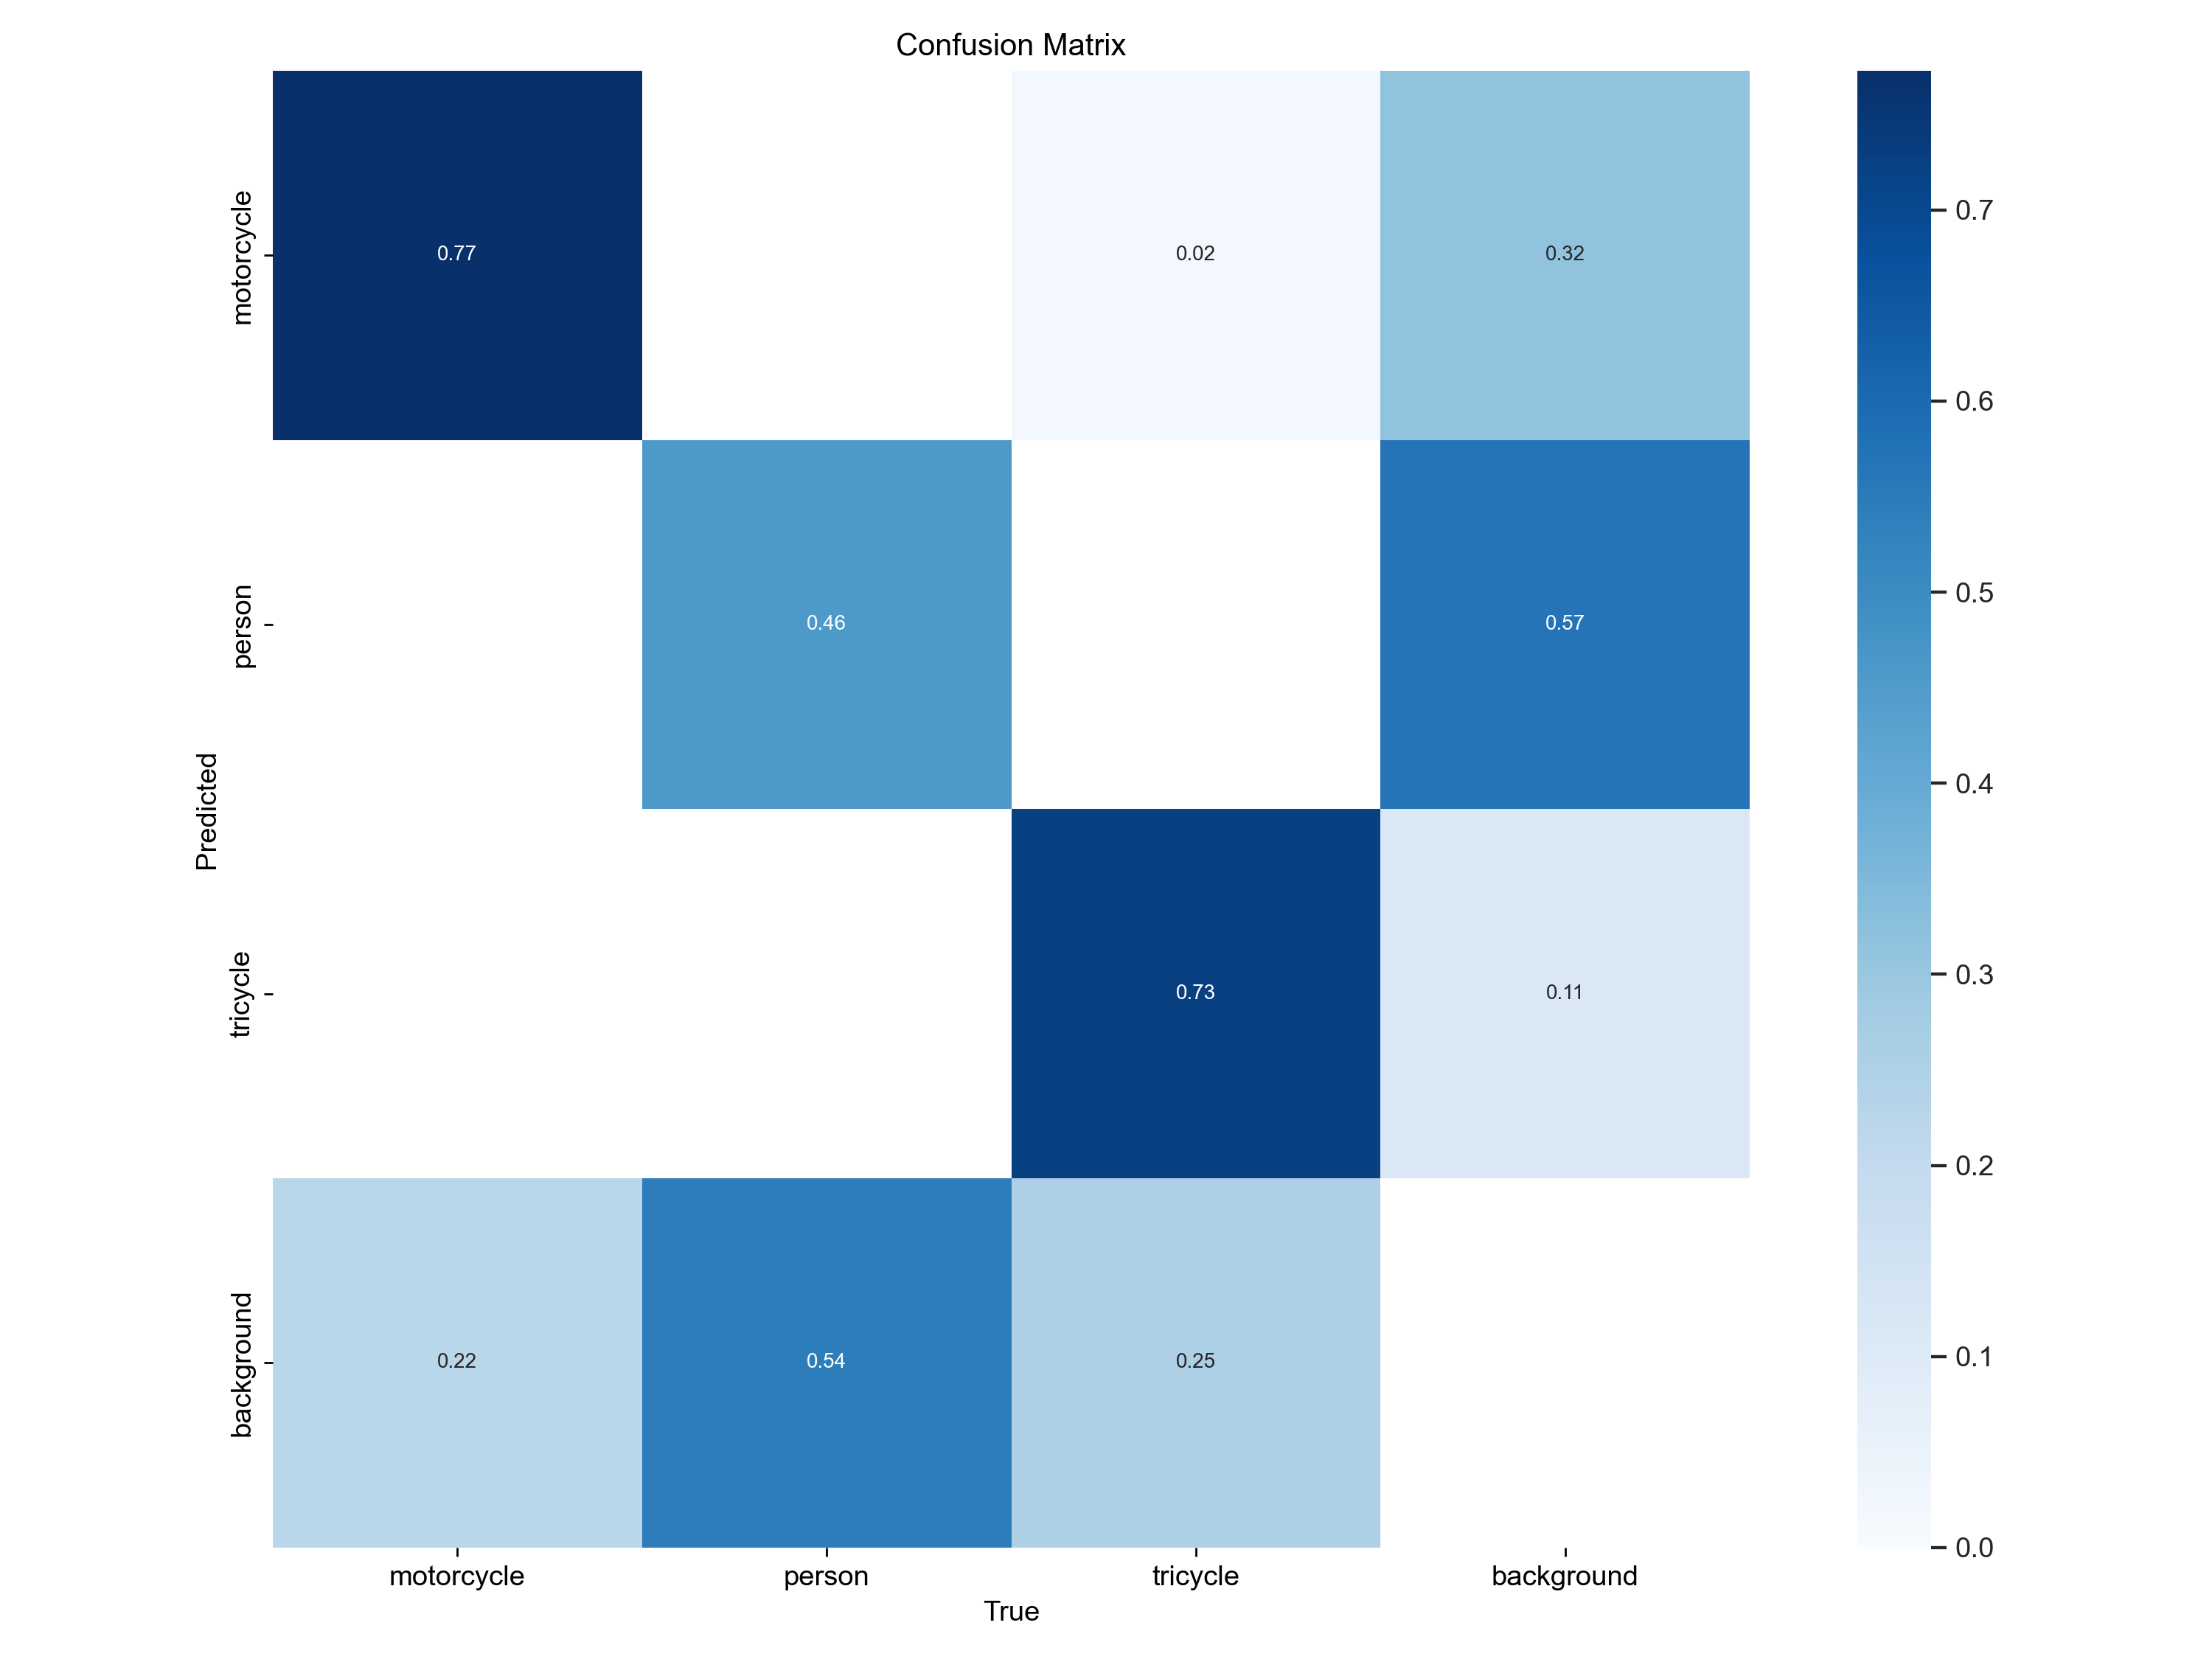
\includegraphics[width=\columnwidth]{Figures/b_confusion_matrix.png}
			\caption{Dataset B: Confusion Matrix of YOLOv5 model}
			\label{fig:mtpDatasetYolov5LargeWeight}
		\end{figure}

\section{Current Findings}
	The following images of~\ref{fig:detectionOfMotorcycleW1},~\ref{fig:detectionOfMotorcycleW2} and~\ref{fig:detectionOfMotorcycleW3} show different wet condition scenarios. Due to previous research conducted, according to Tesla, ``Tesla announces in 2021 that the company would remove a sensor called Ultrasonic Sensors, replacing the sensor with `Tesla Vision' by 2022''.~\cite{noauthor_tesla_nodate} This only means according to ``Self-Driving Cars and The Law: Putting autonomous vehicles on the road isn't just a matter of fine-tuning technology'' by Nathan A. Greenblatt, that AVs used `...thanks to lidar, radar, and ultrasonic sensors, they can see through fog and in the dark.', meaning that Tesla AVs for example, only use visual aid to see. However, this raises concerns about the reliability of Tesla's AVs that solely use visual input. For instance, in situations where the camera's view might be obscured by wet patches or heavy fog, a human driver could potentially outperform the technology.

	Image of a motorcycle in wet weather condition, the architecture trained weight has successfully found the motorcycle with 75\% positiveness that it is a motorcycle. 
	\begin{figure}[htp]
        \centering
        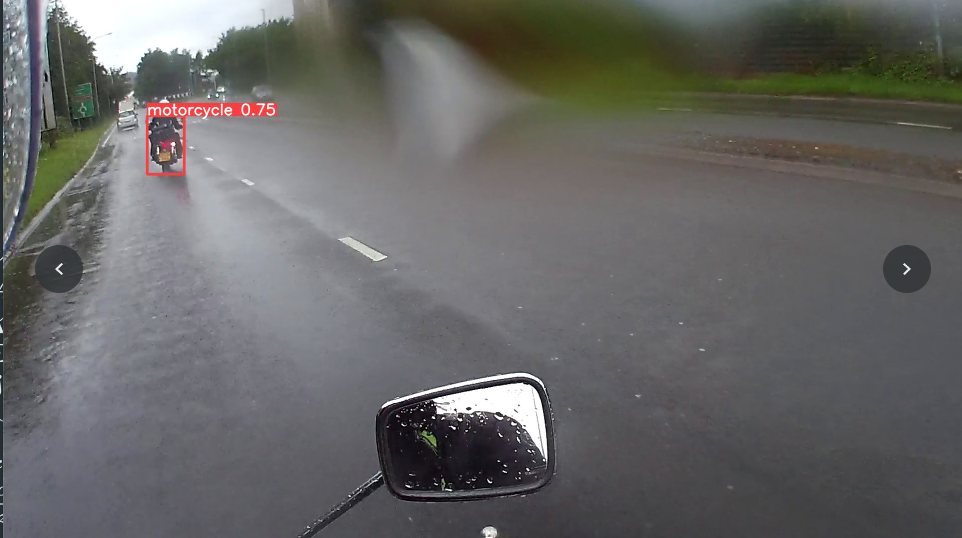
\includegraphics[width=\columnwidth]{Figures/wet_correct.png}
        \caption{Good Detection of Motorcycle - Wet and Multi Lane}
        \label{fig:detectionOfMotorcycleW1}
    \end{figure}

	Image of a motorcycle in wet weather condition, the architecture failed to find the motorcycle. This happened when the camera was blurred from the water content, which could simulate current problems with vision technology within AVs.
	\begin{figure}[htp]
        \centering
        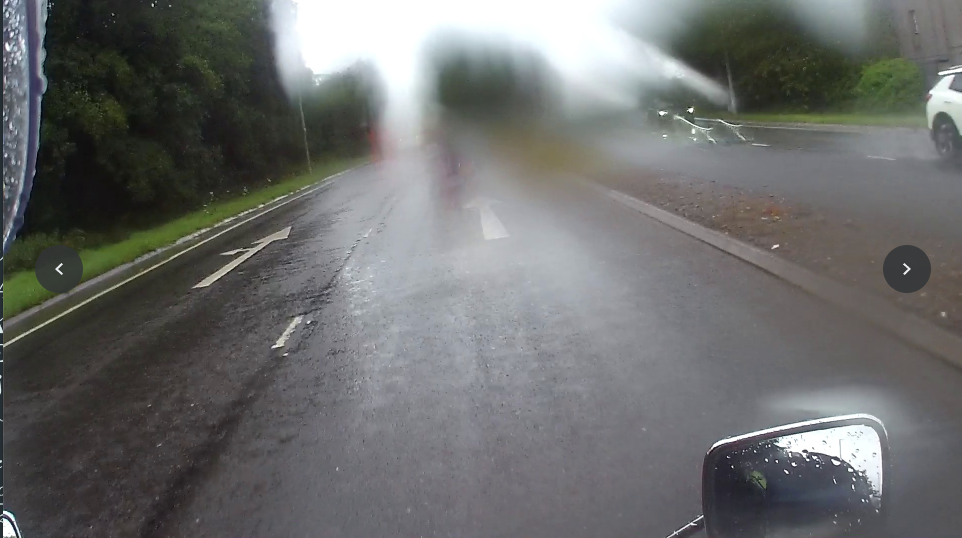
\includegraphics[width=\columnwidth]{Figures/wet_incorrect.png}
        \caption{Classification Error - Camera Blinded}
        \label{fig:detectionOfMotorcycleW2}
    \end{figure}

	Image of a motorcycle in wet weather condition, the architecture failed to find the motorcycle. The visibility is moderate, human eyesights could easy see more than eight to ten meters ahead. Another observation of this footage was that the vehicles are visible, although, the architecture failed to recognise the motorcycle.
	\begin{figure}[htp]
        \centering
        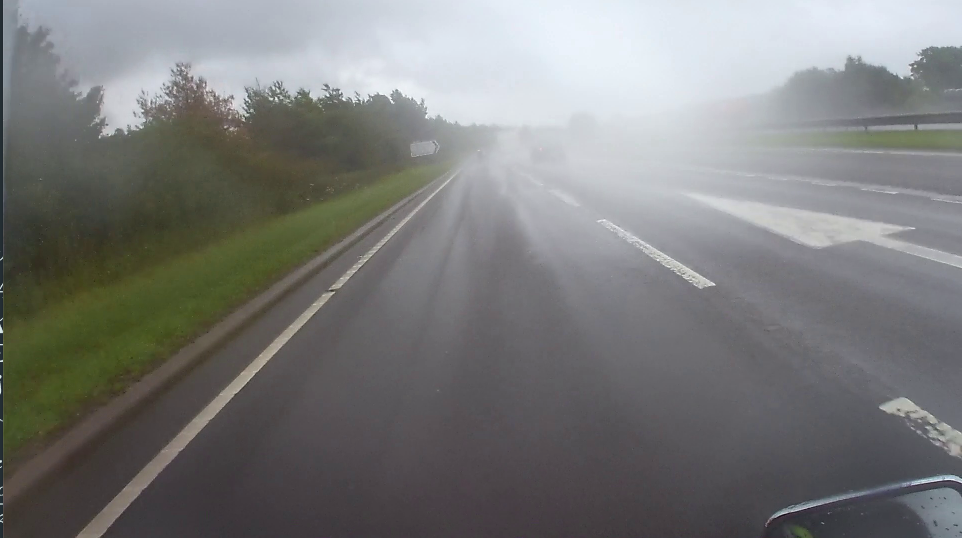
\includegraphics[width=\columnwidth]{Figures/wet_danger.png}
        \caption{Classification Error - Camera Blinded}
        \label{fig:detectionOfMotorcycleW3}
    \end{figure}

\section{Discussion}
	
\section{Conclusion}

\section{Further Research}
	After reviewing some of the findings so far within the research, it imposes some serious questions, such as `Will an AV detect a motorcycle at last minute, having to emergency break when it had plenty of time beforehand?', `Can a AV turn in the path of a motorcycle with current blindspot risks?' and `Can motorcyclists do more to get in safer positions when AVs are on the UK roads?'. These questions will expand the leading dissertation research, helping to ask many unanswered questions or draw attention to a perhaps overlooked subject area of AV development.

\section{Terminology}
	List of terminologies used in this document:-
	\begin{itemize}
		\item AV - Autonomous Vehicles.
	\end{itemize}

%\nocite{*}
\renewcommand\refname{\section{Reference List}}
\small{\bibliographystyle{IEEEtran}
	\bibliography{ref}}
\end{document}